
\documentclass[11pt]{article}

\usepackage{common}
\title{HW3: Language Modeling}
\author{Jeffrey Ling \\ jling@college.harvard.edu \and Rohil Prasad \\ prasad01@college.harvard.edu }
\begin{document}

\maketitle{}
\section{Introduction}

In this assignment, we examine the problem of language modeling. Given a set of words, we want to determine which word comes after it. Note, however, that there may not be a ``best'' word to follow a prefix. For example, ``fish'' and ``chicken'' could both be almost equally likely to follow the prefix ``I ate \_\_\_''. Therefore, it makes more sense to try and find a good \textbf{probability distribution} of the next word given the prefix. We will define what it means to be ``good'' later in the paper. 

We implement and discuss several different methods of language modeling on the Penn Treebank in this paper. Our first class of algorithms are probabilistic count-based algorithms, consisting of maximum likelihood estimation, Laplace smoothing, Witten-Bell smoothing, and Kneser-Ney smoothing. Our second class of algorithms are deep-learning algorithms, consisting of the neural network described in [Bengio]. Furthermore, we also experiment with augmenting this neural network with word embeddings learned via Noise Contrastive Estimation (NCE). 

In Section 2, we give a formal description of our problem and establish our notation. In Section 3, we give detailed descriptions of the algorithms listed above. In Section 4, we present our experimental results. In Section 5, we discuss our findings. 

\section{Problem Description}

Assume our training corpus consists of a sequence of words $w_1, w_2, \dots, w_N$ where $w_i$ is drawn from a vocabulary $\mathcal{V}$ for every $i$. 

Our training data represents this corpus as a set of tuples $(\mathbf{x}_i, y_i)$, where $\mathbf{x}_i$ is the prefix $w_1w_2\dots w_{i-1}$ and $y_i$ is equal to the suffix $w_i$. 

Our goal is to train a model that will take in an input sequence $\mathbf{x}$ of words and output a vector $\mathbf{y} \in \mathbb{R}^{1 \times |\mathcal{V}|}$ where $\mathbf{y}_i = p(v_i | x)$ for $v_i$ the $i$th element of $|\mathcal{V}|$.

\subsection{Count-Based Model Notation}

We use some specific notation for our count-based models. 
\begin{itemize}
  \item $w^{i-1}_{i-n+1}$ is our shorthand for the size $n-1$ prefix $w_{i-n+1}w_{i-n+2}\dots w_{i-1}$ of $w_i$. When $n = 2$, we will continue to use $w_{i-1}$. 
  \item $c(w_i)$ denotes the total number of occurrences of the word $w_i$ in the training corpus. 
  \item $c(w^{i-1}_{i-n+1}, w_i)$ denotes the total number of occurrences of the word $w_i$ after the prefix $w^{i-1}_{i-n+1}$ in the training corpus. 
  \item $N(\cdot, w_i)$ denotes the total number of unique prefixes of size $n$ that $w_i$ has in the training corpus. 
  \item $N(w^{i-1}_{i-n+1}, \cdot)$ denotes the total number of unique suffixes that the sequence $w^{i-1}_{i-n+1}$ has in the training corpus. 
\end{itemize}

\subsection{Evaluation}

Unlike earlier assignments, we are outputting a \emph{distribution} of possibilities given an input $\mathbf{x}$ rather than a \emph{prediction} of the word following $\mathbf{x}$. 

Therefore, we will evaluate by a metric called \emph{perplexity}. This is equal to the exponent of the average negative log-likelihood over all of our samples:
$$e^{-\frac{1}{n}\sum_{i=1}^n \log p(y = y_i | x_i)}$$

\section{Model and Algorithms}

\subsection{Count-Based Models}

All of our count-based models are $n$-gram models, meaning we fix an $n$ and assume $p(w_i|w^{i-1}_1) = p(w_i|w^{i-1}_{i-n+1})$. 

\subsubsection{Maximum Likelihood Estimation}

The maximum likelihood estimation $p_{MLE}(w_i|w^{i-1}_{i-n+1})$ is given by 
$$p_{MLE}(w_i|w^{i-1}_{i-n+1}) = \frac{c(w^{i-1}_{i-n+1}, w_i)}{\sum_{w' \in \mathcal{V}} c(w^{i-1}_{i-n+1}, w')}$$

This is by definition the probability over the training corpus of the word $w_i$ appearing conditioned on the prefix being equal to $w^{i-1}_{i-n+1}$. 

\subsubsection{Laplace Smoothing}

 One thing to note is that our MLE model will by definition assign a (clearly erroneous) probability of $0$ to $p(w|w^{i-1}_{i-n+1})$ for any $w^{i-1}_{i-n+1}$ that does not appear in the training corpus. This poses a problem for larger $n$, since the number of distinct $n$-grams in the training corpus will only form a small fraction of the number $|\mathcal{V}|^n$ of possible $n$-grams.

The traditional maximum likelihood $n$-gram model by definition will often erroneously assign a probability of $0$ to $p(w|w^{i-1}_{i-n+1})$. 

We fix this by adding $\alpha$ to the count of every word. Then, our probability becomes 
$$p_L(w_i|w^{i-1}_{i-n+1}, \alpha) = \frac{\alpha + c(w^{i-1}_{i-n+1}, w_i)}{\alpha \cdot |\mathcal{V}| + \sum_{w' \in \mathcal{V}} c(w^{i-1}_{i-n+1}, w')}$$

The optimal value for $\alpha$ is determined by grid search on a validation set. 

\subsubsection{Witten-Bell Smoothing}

The Witten-Bell probability for bigrams with an additive smoothing parameter $\alpha$ is written as

$$p_{WB}(w_i|w_{i-1}) = \lambda_{w_{i-1}} p_L(w_i|w_{i-1}, \alpha) + (1-\lambda_{w_{i-1}}) p_L(w_i| \alpha)$$

where $\lambda_{w_{i-1}}$ is determined by the following equation:

$$1 - \lambda_{w_{i-1}} = \frac{N(w_{i-1}, \cdot)}{N(w_{i-1}, \cdot) + c(w_{i-1}, w_i)}$$

We can then define Witten-Bell recursively for $n$-grams as

$$p_{WB}(w_i|w^{i-1}_{i-n+1}) = \lambda_{w^{i-1}_{i-n+1}} p_L(w_i|w^{i-1}_{i-n+1}, \alpha) + (1-\lambda_{w^{i-1}_{i-n+1}}) p_{WB}(w_i|w^{i-1}_{i-n+2})$$

where $\lambda_{w^{i-1}_{i-n+1}}$ is given by:

$$1 - \lambda_{w^{i-1}_{i-n+1}} = \frac{N(w^{i-1}_{i-n+1}, \cdot)}{N(w^{i-1}_{i-n+1}, \cdot) + c(w_i, w^{i-1}_{i-n+1})}$$ 

The optimal value for $\alpha$ is determined by grid search on a validation set. 

\subsubsection{Kneser-Ney Smoothing}

For Kneser-Ney, we define the lower-order probabilities as follows. Fix a ``discount parameter'' $\delta$. For unigrams, the equation is:

$$p_{KN}(w_i) = N(\cdot, w_i)/\sum_{w' \in \mathcal{V}} N(\cdot, w')$$

Then for bigrams, it is defined as 

$$p_{KN}(w_i | w_{i-1}) = \frac{\text{max}(c(w_{i-1}, w_i) - \delta, 0)}{\sum_{w' \in \mathcal{V}} c(w_{i-1}, w')}$$

Finally, we can define it recursively for general $n$-grams:

$$p_{KN}(w_i | w^{i-1}_{i-n+1}) = \frac{\text{max}(c(w^{i-1}_{i-n+1}, w_i) - \delta, 0)}{\sum_{w' \in \mathcal{V}}c(w^{i-1}_{i-n+1}, w')}$$

The optimal value for $\delta$ is determined by grid search on a validation set. 

\subsection{Neural Network Model}

\subsection{Noise Contrastive Estimation}

\section{Experiments}

\subsection{Count-Based Models}

For our count-based models, we noticed that the perplexity of Laplace smoothing and Witten-Bell smoothing on our validation set were sensitive to the hyperparameter $\alpha$ from a few random tests. Therefore, we did an exhaustive grid-search, running over $\alpha = n \cdot 10^{-k}$ for $1 \leq n \leq 9$ and for several $k$. 

We graph perplexity on the validation set for Laplace smoothing and Witten-Bell smoothing for both bigrams and trigrams. 

Laplace smoothing perplexity is graphed for $\alpha = n \cdot 10^{-k}$ for $k \in \{-4, -3, -2, -1\}$ while Witten-Bell smoothing perplexity is graphed for $\alpha = n \cdot 10^{-k}$ for $k \in \{-4, -3, -2\}$. The data for $k = -1$ is cut off in this case to allow easier visualization, as the perplexity starts to increase very quickly past $\alpha = 0.1$.  

We give the optimal $\alpha$ with their corresponding perplexity in a table below. 

\begin{table}[h]
  \centering
  \begin{tabular}{llcc}
    \toprule
    Model & N-gram Size & $\alpha$ & Perplexity \\
    \midrule
    \textsc{Laplace Smoothing} & 2 & 0.008 & 296.877 \\
    & 3 & 0.03 & 398.745 \\
    \textsc{Witten-Bell Smoothing} & 2 & 0.0007 & 215.055 \\
    & 3 & 0.0006 & 368.696 \\
    \bottomrule
  \end{tabular}
  \label{tab:alpha}
\end{table}



\section{Conclusion}

Bye



\appendix

\section{Figures} 

\begin{figure}[f]
  \centering
  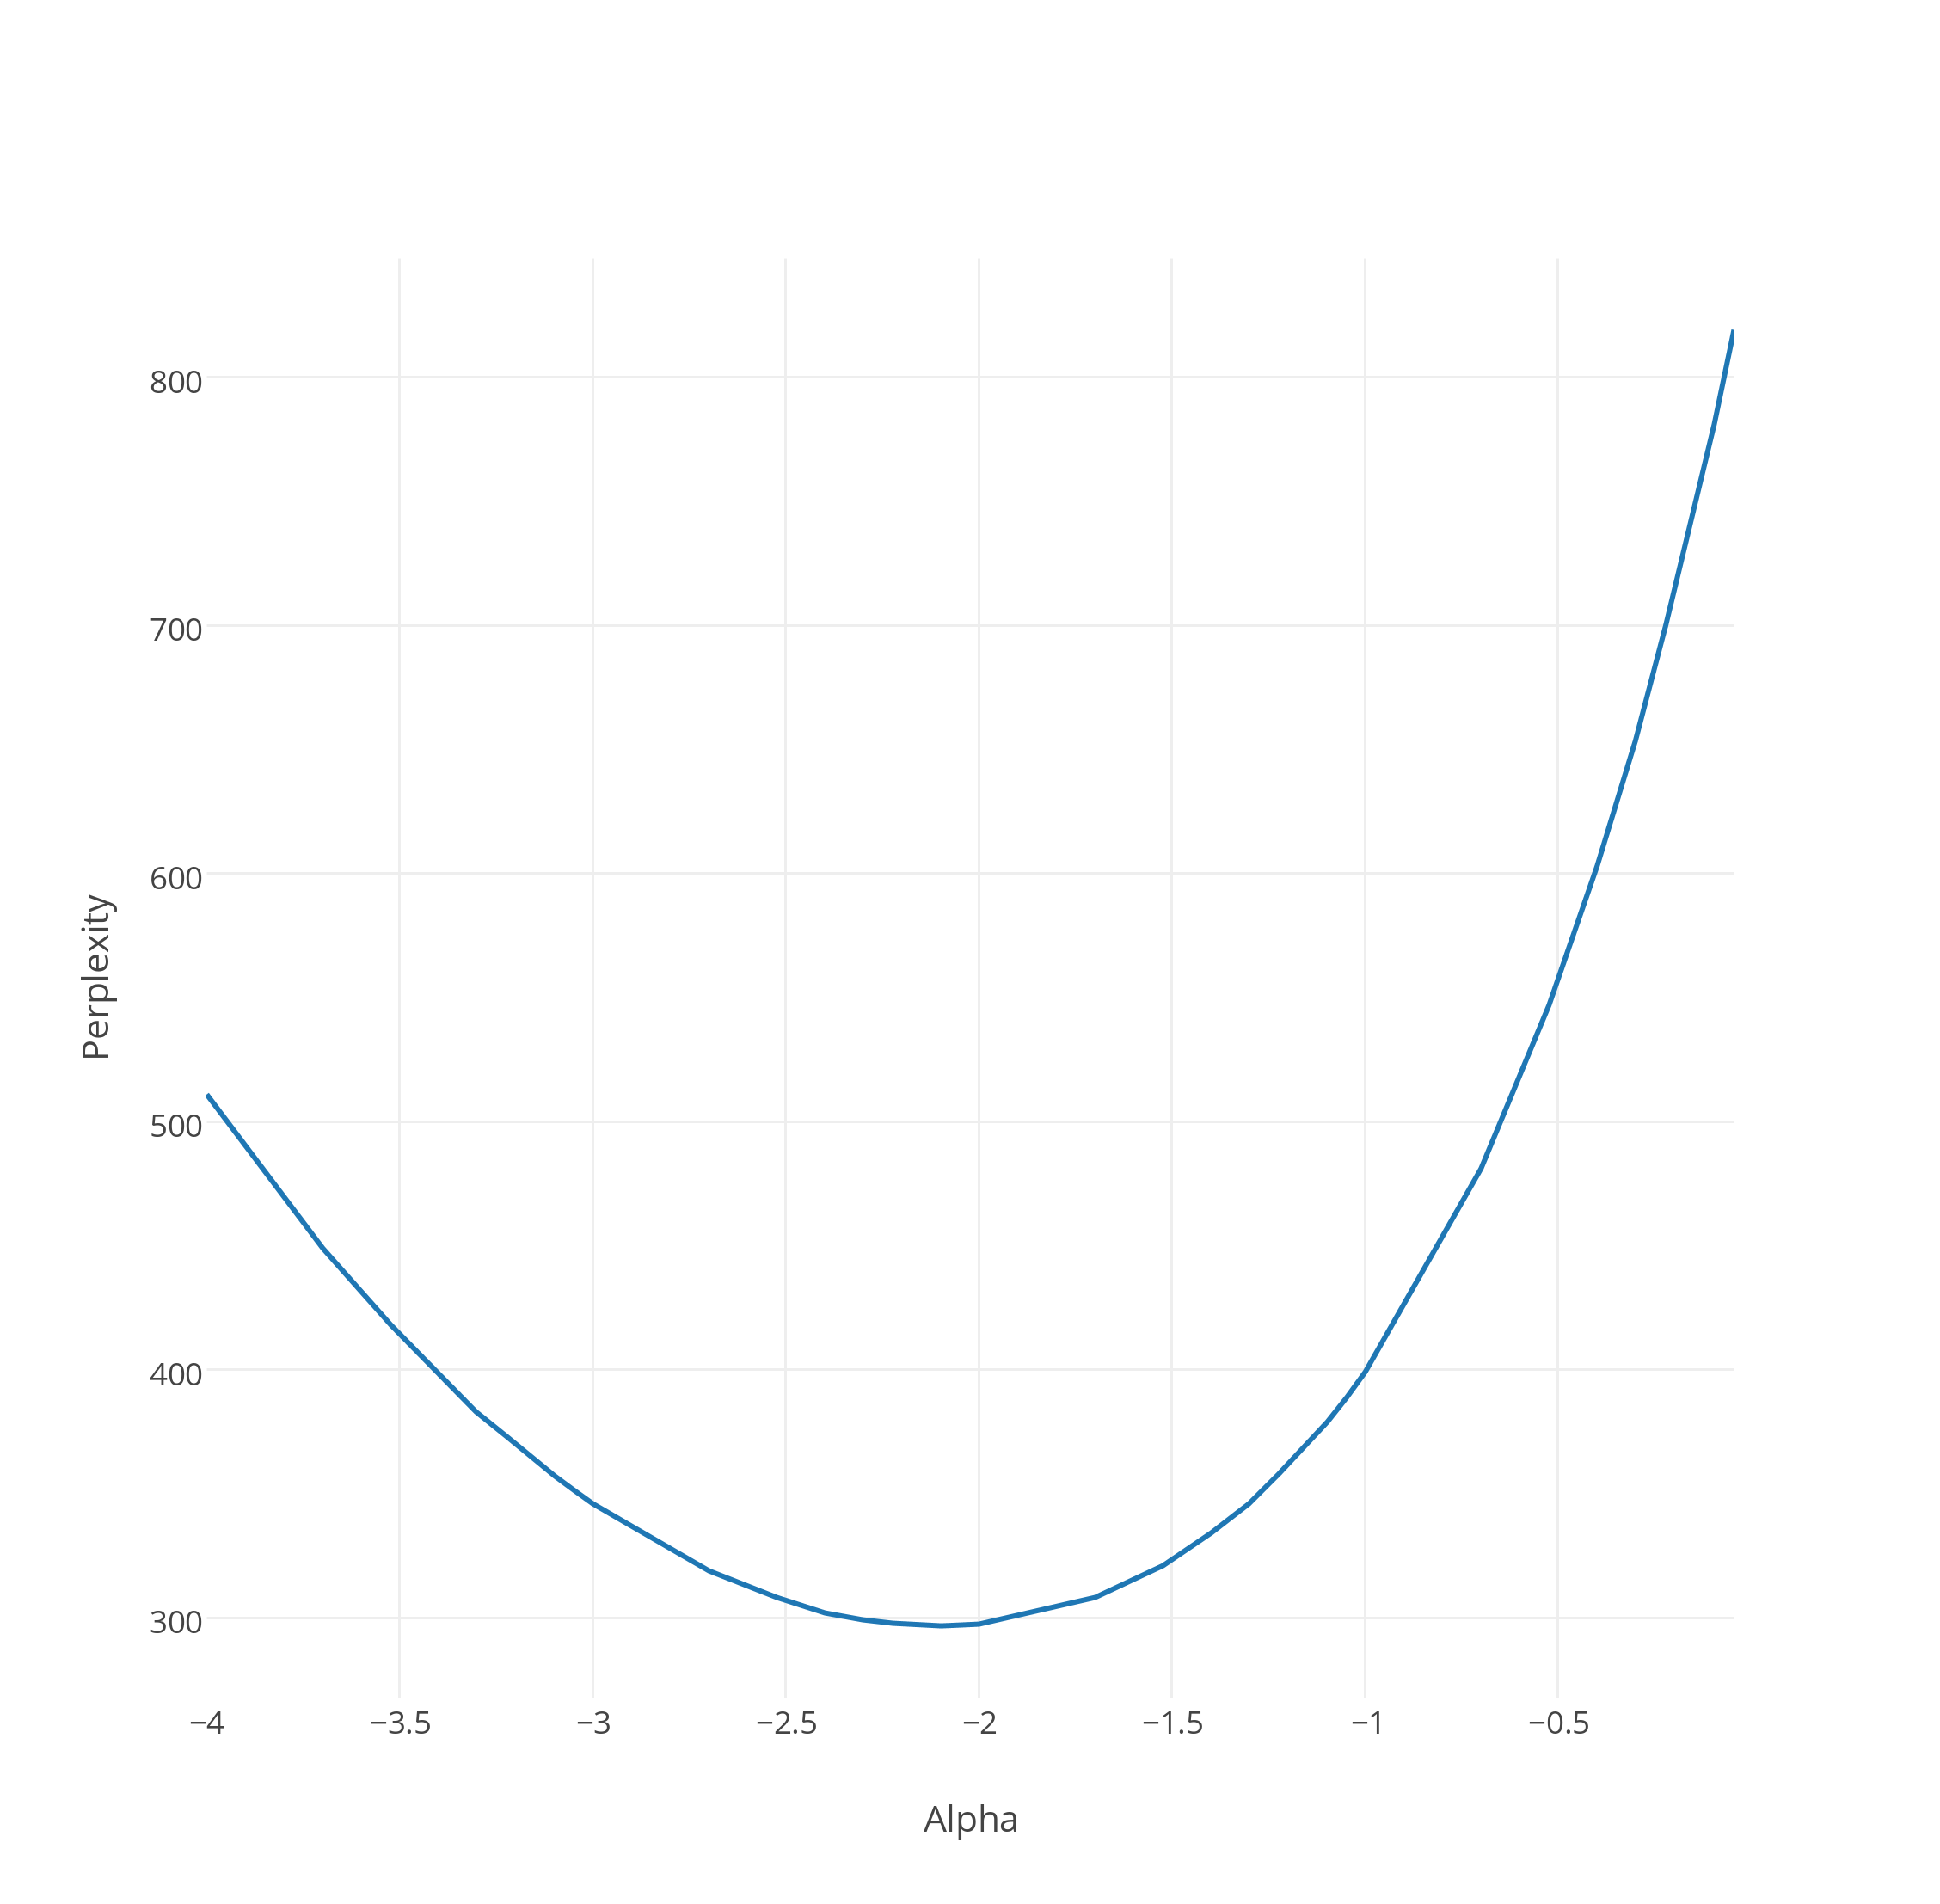
\includegraphics{laplace_2grams.png} \caption{Laplace smoothing for bigrams} \label{fig:laplace2}
\end{figure}


\begin{figure}[f]
  \centering
  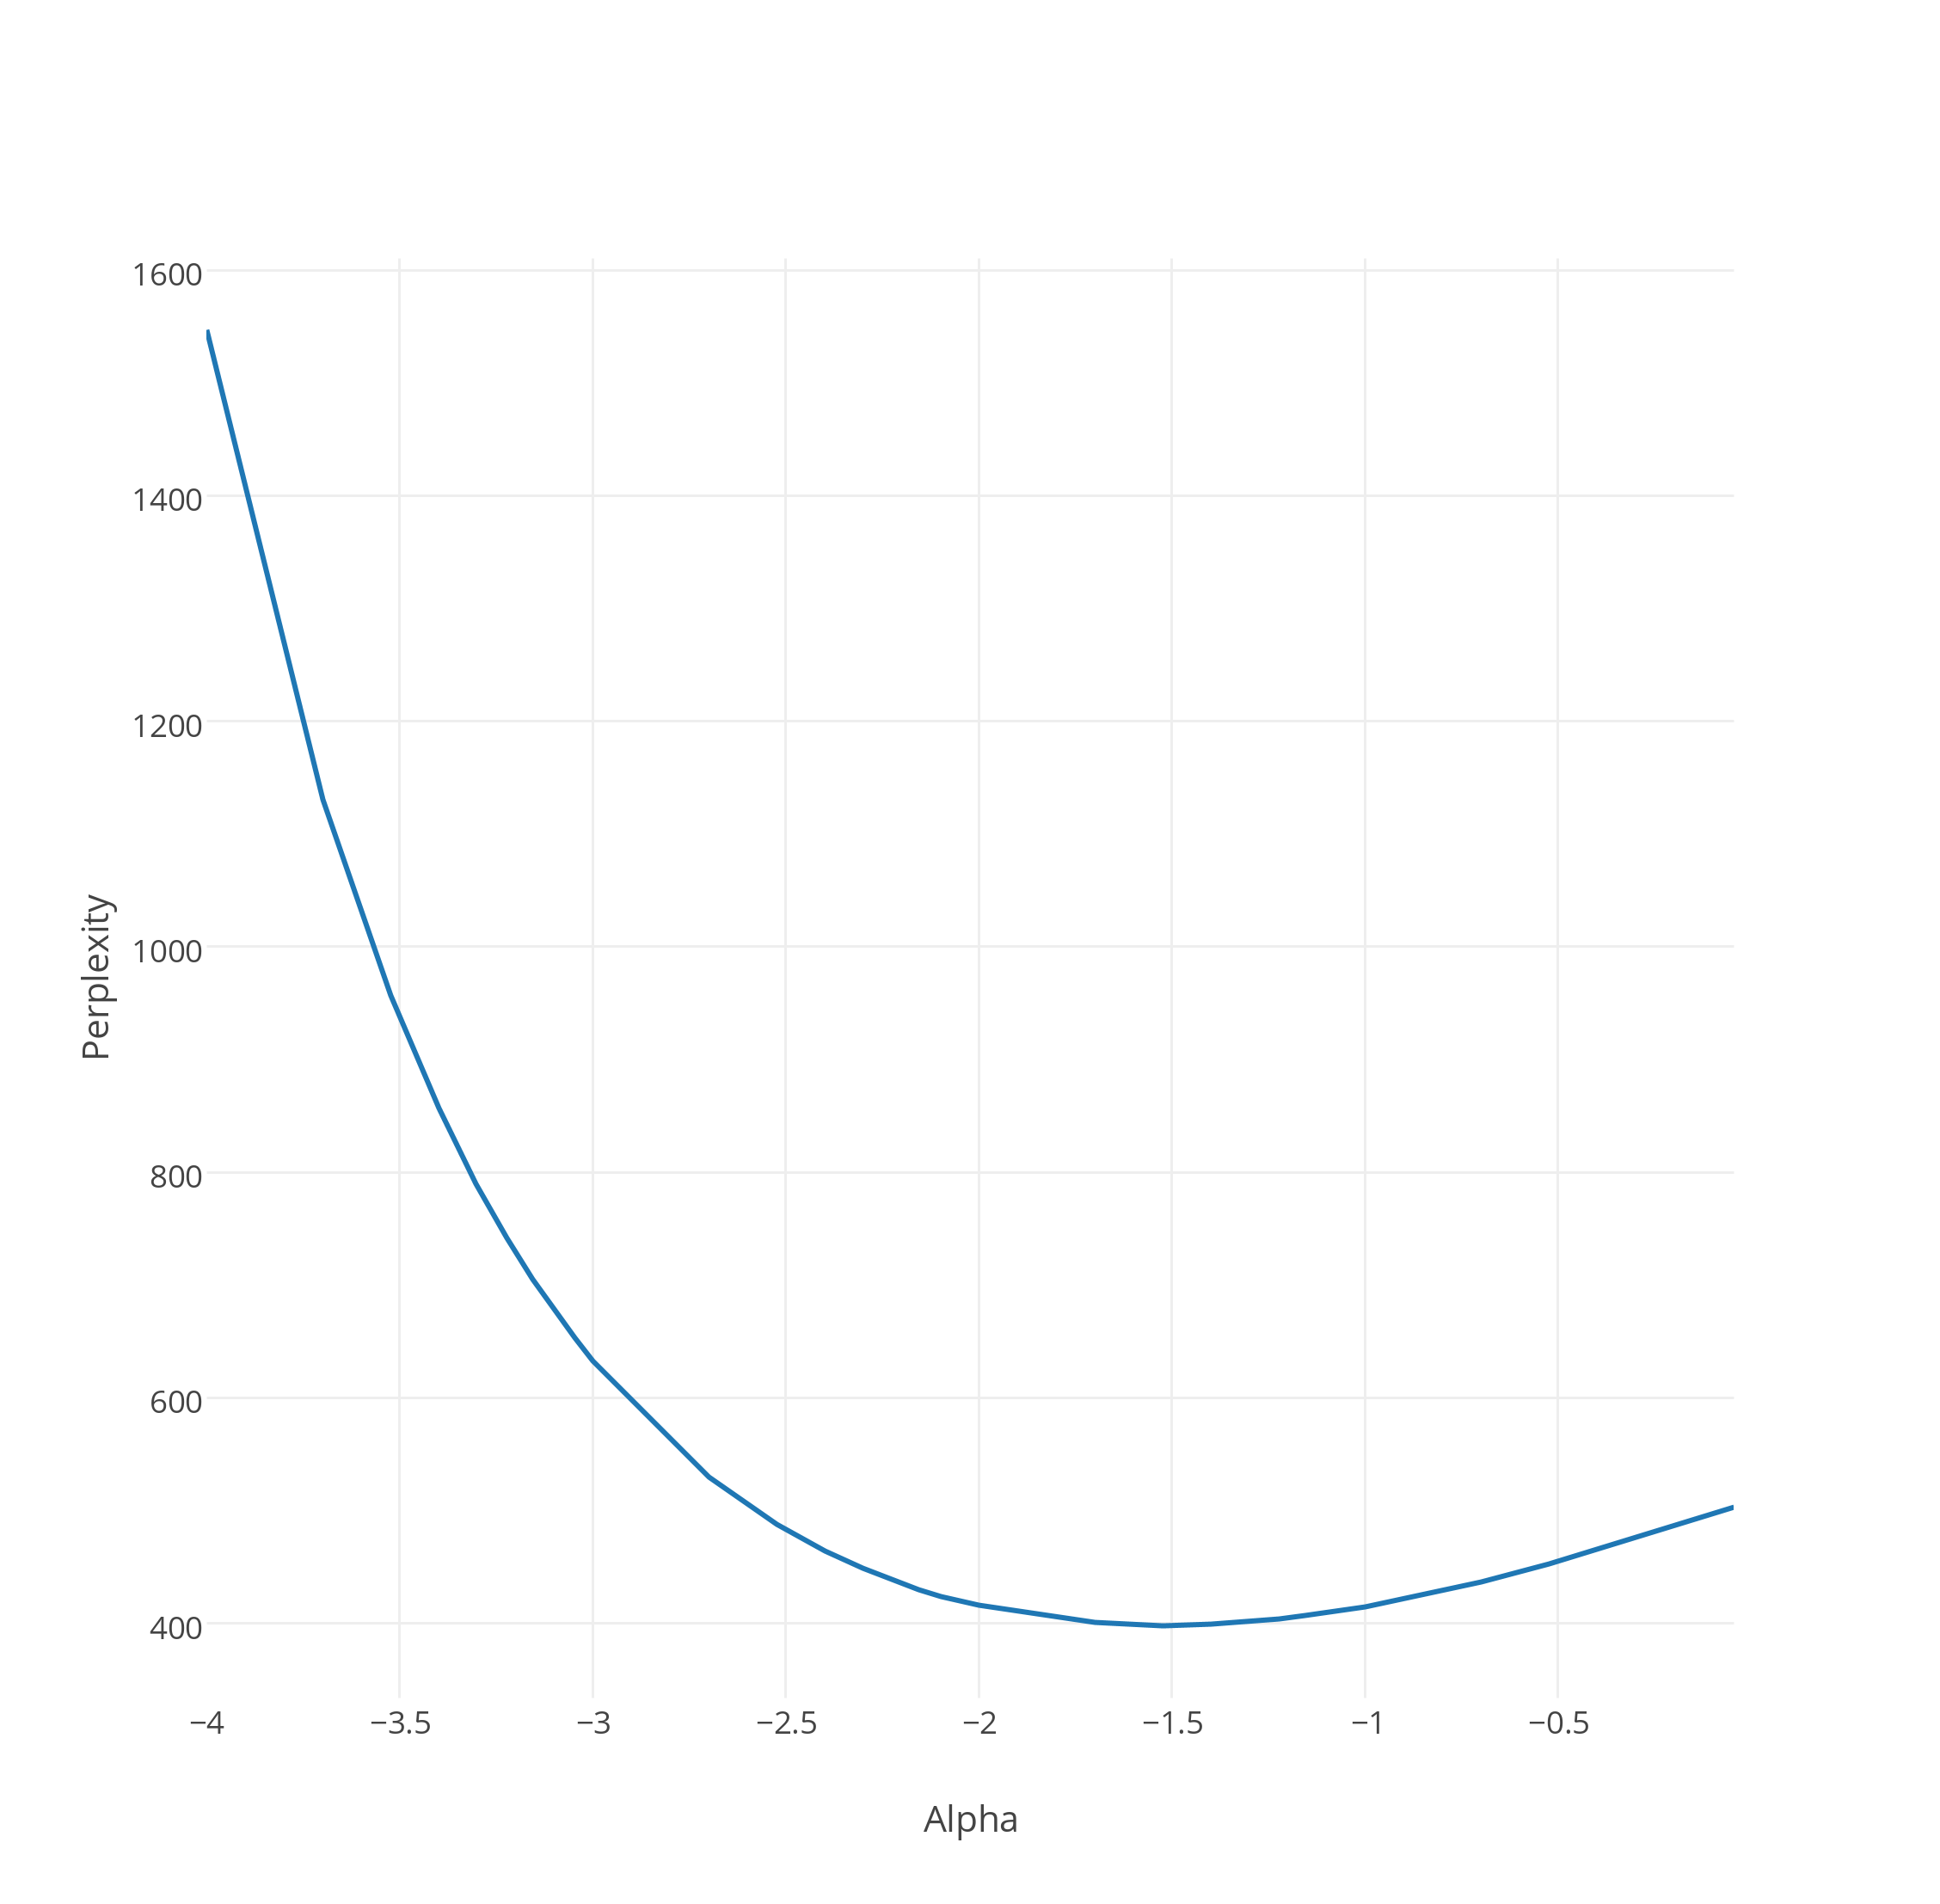
\includegraphics{laplace_3grams.png}
  \caption{Laplace smoothing for trigrams}
  \label{fig:laplace3}
\end{figure}

\begin{figure}[f]
  \centering
  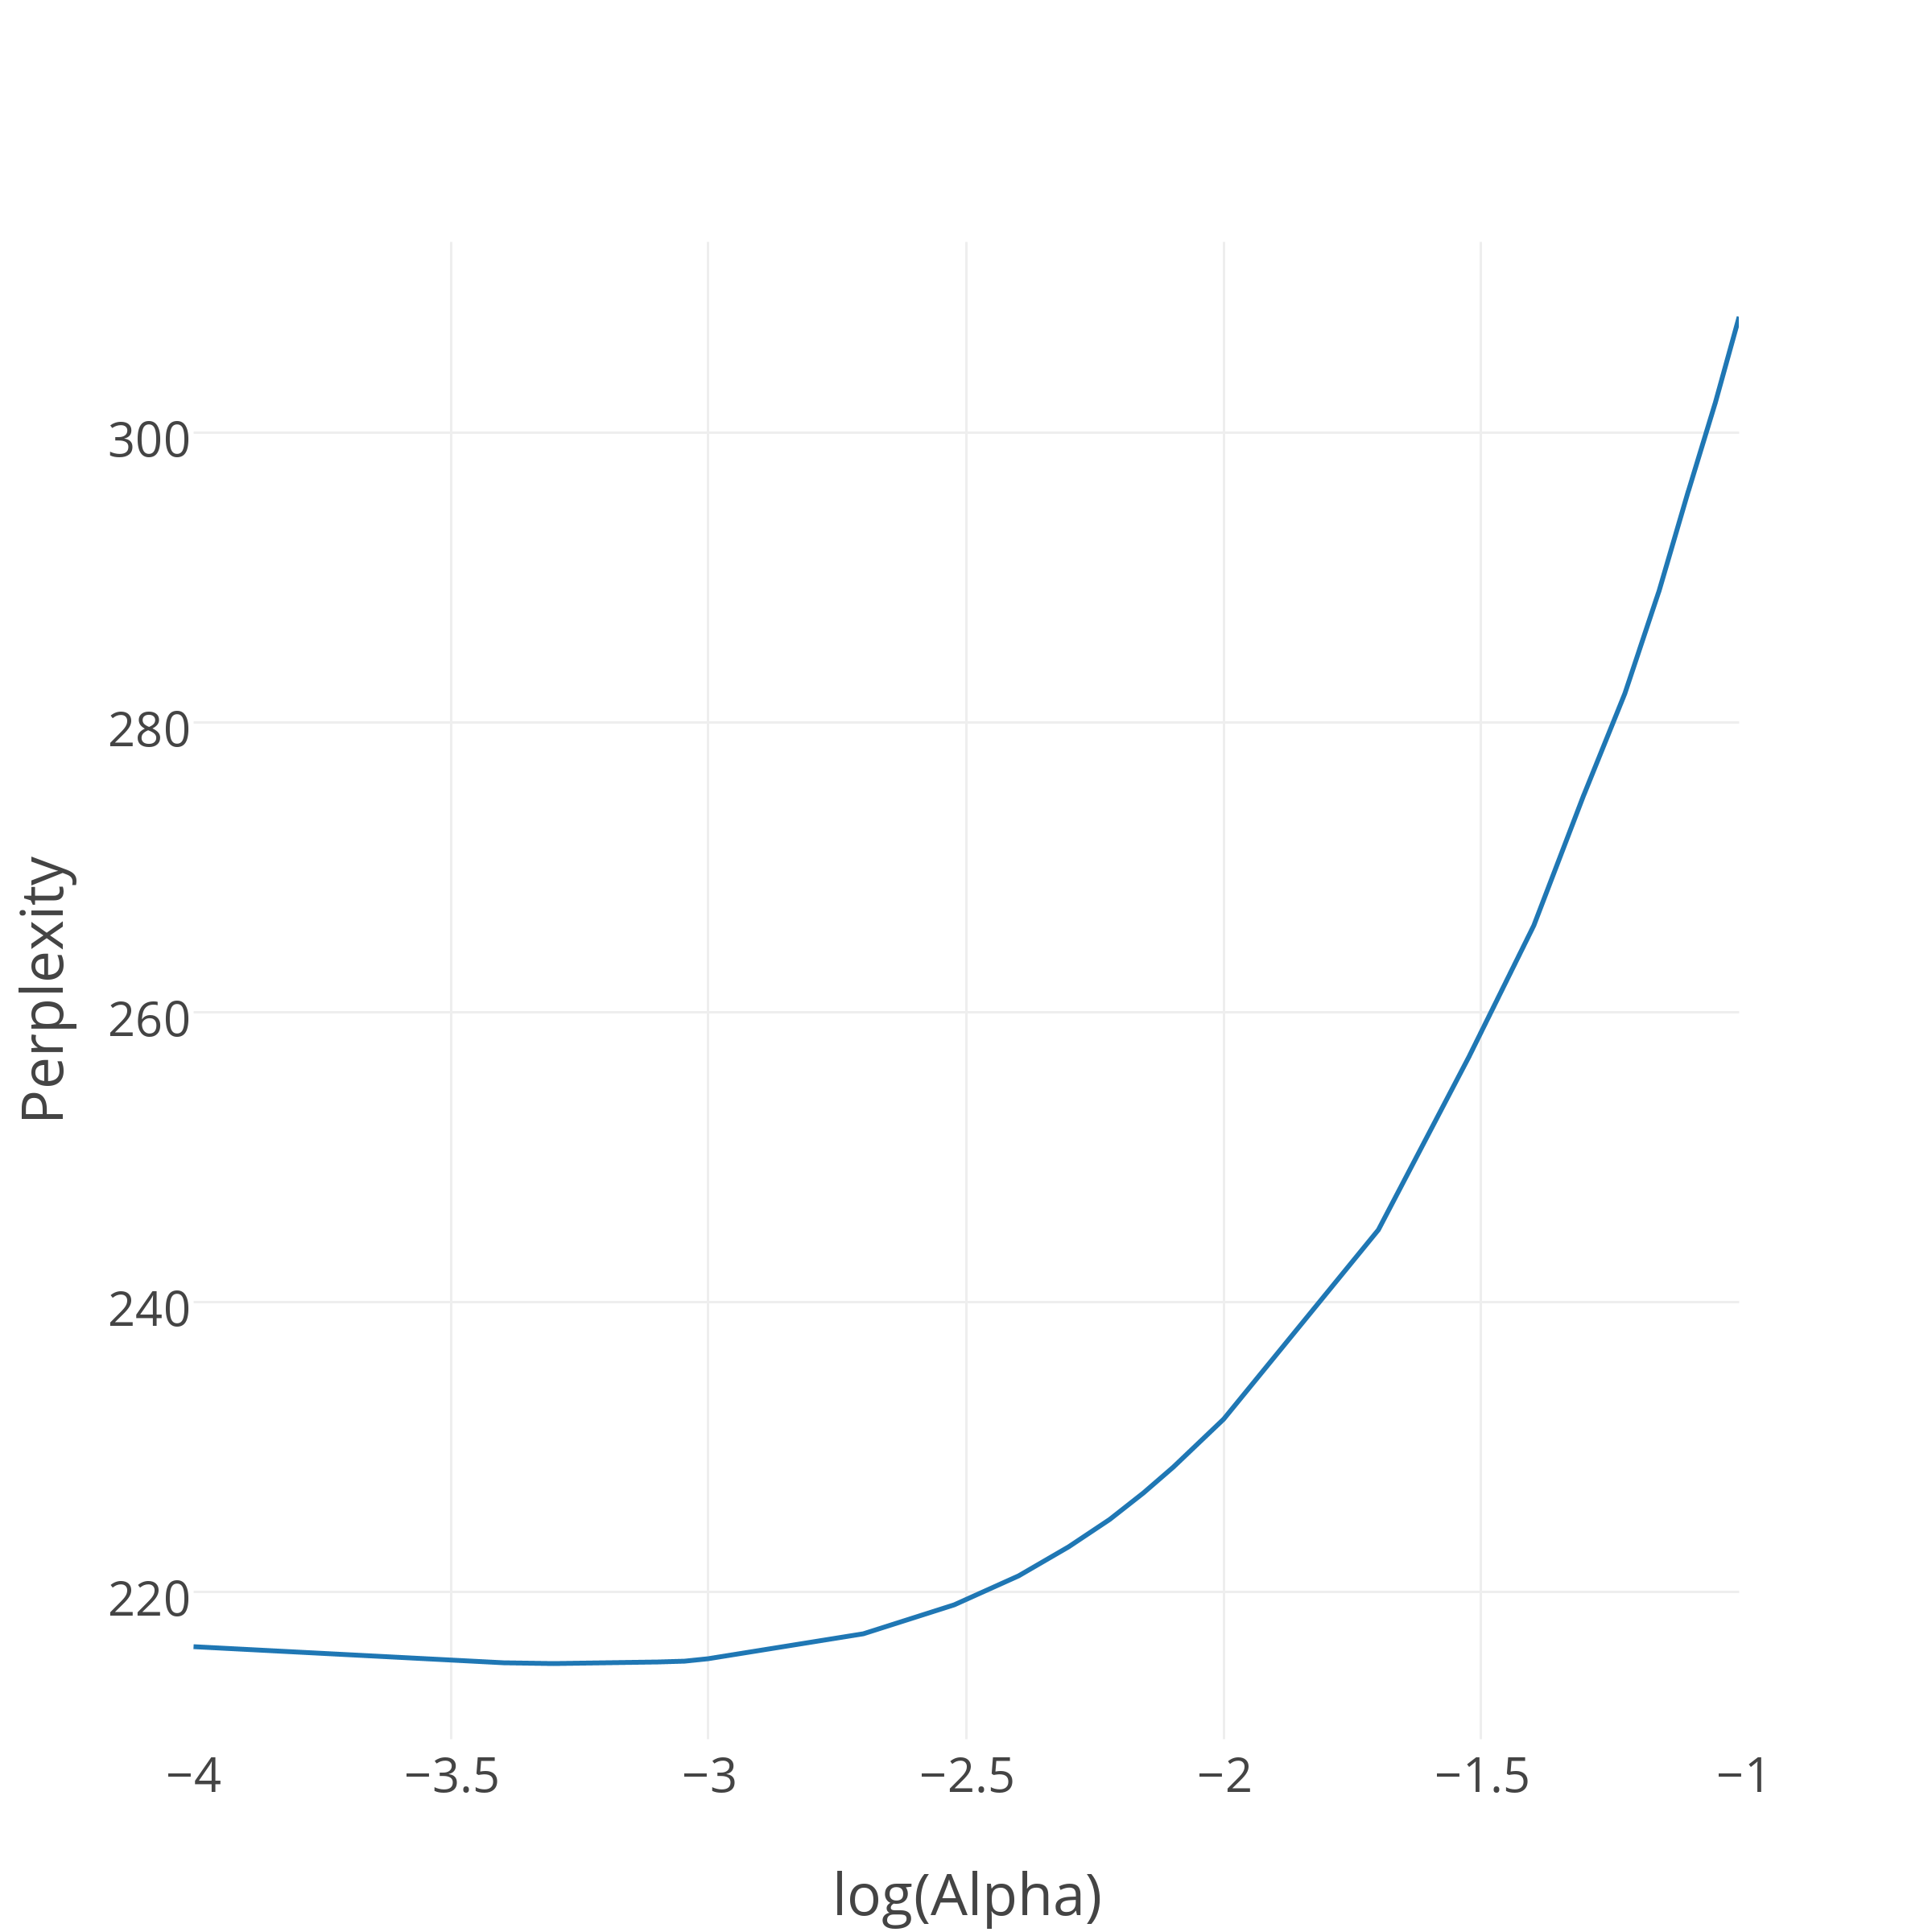
\includegraphics{wb_2grams.png}
  \caption{Witten-Bell smoothing for bigrams}
  \label{fig:wb2}
\end{figure}

\begin{figure}[f]
  \centering
  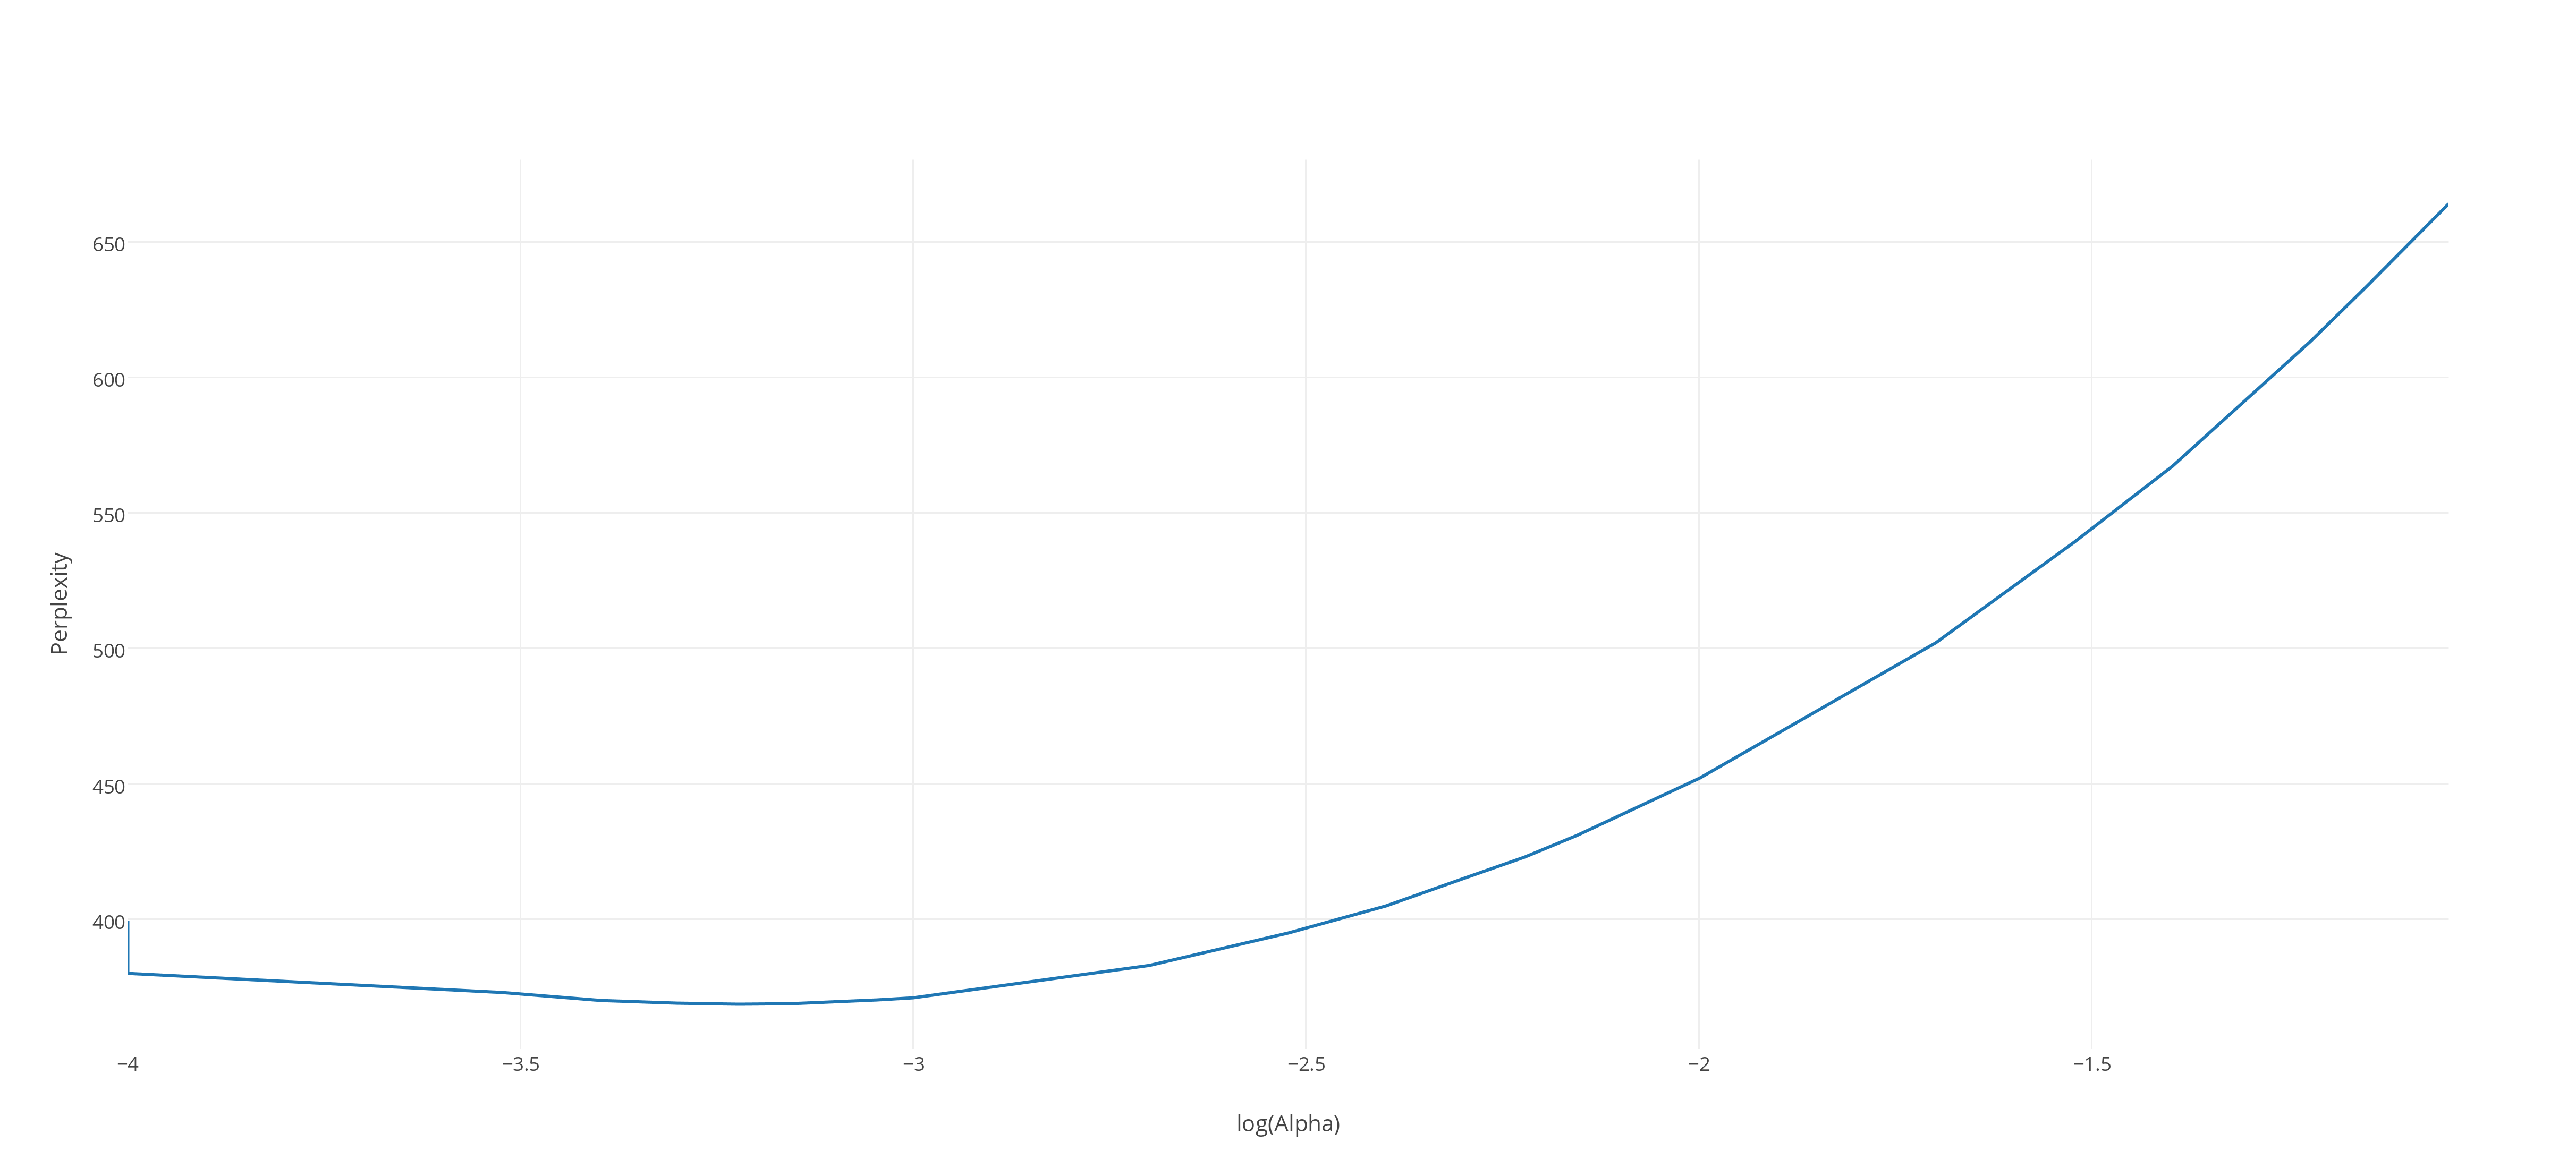
\includegraphics{wb_3grams.png}
  \caption{Witten-Bell smoothing for trigrams}
  \label{fig:wb3}
\end{figure}

%\bibliographystyle{apalike}
%\bibliography{writeup}

\end{document}
